\documentclass[]{msulabm}
\usepackage[utf8]{inputenc}
\usepackage{amsmath}
\usepackage{graphicx}
%\usepackage[linktocpage]{hyperref}  % if not using colorlinks, use linktocpage
\usepackage[colorlinks]{hyperref}  % if not using colorlinks, use linktocpage
\usepackage{bm}            % bold math
\usepackage{multirow}
\usepackage[table]{xcolor} % provide alternating rows with colors
\usepackage{textcomp}
\usepackage{xfrac} % gives split-level fractions with '\sfrac{a}{b}
\usepackage{multicol}
\usepackage[section]{placeins} % provides \FloatBarrier, to keep floats from crossing this barrier
\usepackage{amssymb}
\usepackage{wrapfig} % provides wrapping figures with text.
%\usepackage{enumitem} % gives \begin{enumerate}[resume] to resume counting from previous enumerate
%\usepackage{subfigure}
%\usepackage{tikz} % to draw arrows
\usepackage{xtab} % provides xtabular, tabular environment that spans multiple pages and other awesome things
\usepackage[style=phys,biblabel=brackets,pageranges=false]{biblatex}
\usepackage{pdflscape}
\usepackage{ragged2e}
\usepackage{longtable}
\usepackage{mathabx} % gives astronomy symbols like \Earth
\usepackage{pdfpages}

\bibliography{references-manual,bbarker-zotero}

\newcommand{\abs}[1]{\left\lvert#1\right\rvert}

\title{Laboratory Manual}
\author{PHSC 12720 Exoplanets \\ \\ The University of Chicago}
\date{Spring 2019}

\pagestyle{ruled}

\definecolor{lgray}{rgb}{.2,.2,.2}

\makeevenfoot{ruled}{\thepage}{\footnotesize{\textit{Last updated \today}}}{}
%\makeevenfoot{ruled}{\thepage}{}}{}
\makeoddfoot{ruled}{}{\color{lgray} \tiny{This work is licensed under \href{http://creativecommons.org/licenses/by-sa/4.0/}{CC BY-SA 4.0} by \href{mailto:bbarker@uchicago.edu}{the University of Chicago}.}}{\thepage}


% allows us to use subcaptions from the memoir class in figures. See Memoir Section 10.9
\newsubfloat{figure}

% don't worry so much about filling every page.
%\raggedbottom

% raise the penalty for splitting footnotes across different pages. Default is 100.
\interfootnotelinepenalty=10000

%\includeonly{amplifier/amplifier} 

% creates a standard length to use 
\newlength{\answerskip}
%\setlength{\answerskip}{90pt} 

%% use plus / minus if latex is squeezing the answer space too much
\setlength{\answerskip}{2cm plus 0.2cm minus 0.2cm}

\newlength{\qaskip}
\setlength{\qaskip}{\answerskip}
\addtolength{\qaskip}{\baselineskip}

% reduce vertical space between chapters in table of contents. Default is 2em.
\setlength{\cftbeforechapterskip}{1em}

% allow for extra line on a page to help prevent widow/orphan lines.
\sloppybottom

% Now we can caption a table outside of the table float environment (good for multi-page tables)
\newfixedcaption{\freetabcaption}{table}

%\includeonly{snells-law/snells-law}
%\includeonly{ohms-law/ohms-law}

\begin{document}
\maxtocdepth{chapter}

 % start roman numbering
 \frontmatter

\maketitle

%\clearpage

%Brent W. Barker

%Department of Astronomy \& Astrophysics

%The University of Chicago

%5640 South Ellis Ave.

%Chicago, IL 60637

%\href{mailto:bbarker@uchicago.edu}{bbarker@uchicago.edu}

%\vspace{2\baselineskip}

%\includegraphics{cc-by-sa-88x31}

%\textcopyright{} 2018 Brent W. Barker. Except where otherwise noted, this work is copyrighted under the Creative Commons Attribution-ShareAlike International 4.0 License. To view a copy of this license, visit \url{http://creativecommons.org/licenses/by-sa/4.0/}.

%\vspace{\baselineskip}

%These labs, excluding "Impulse and Momentum" and the appendices, are a derivative of "\href{https://%sites.google.com/site/scientificabilities/ISLE-labs}{ISLE Labs}" by the Rutgers Physics and Astronomy %Education Research group, used under the Creative Commons Attribution International 4.0 License.
%To view a copy of this license, visit \url{http://creativecommons.org/licenses/by/4.0/}.

%At Rutgers University, many people contributed to this project over the years.
%The list of names is very long and includes: Eugenia Etkina, Alan Van Heuvelen, Suzanne Brahmia, David %Brookes, Michael Gentile, Anna Karelina, Michael Lawrence, Marina Milner-Bolotin, Sahana Murthy, Maria %Ruibal-Villasenor, Aaron Warren, Xueli Zou.

 % skip to next right leaf (``recto'')
 \cleartorecto

 % the star means that the ToC itself is not listed in the ToC
 \tableofcontents*

 % start arabic numbering
\mainmatter 

\chapter{Scale of the solar system and local stellar environment}

%todo for proxima group, add the voyager probes and the heliopause (with info about probes, when sent, etc)

\begin{quotation}
	\textit{Space is big. You just won't believe how vastly, hugely, mind-bogglingly big it is. I mean, you may think it's a long way down the road to the chemist's, but that's just peanuts to space.} \sourceatright{Douglas Adams, The Hitchhiker's Guide to the Galaxy}
\end{quotation}

Why can't we just see planets orbiting other stars with normal observational techniques like looking through larger and larger telescopes? Through this lab, we hope you gain a felt sense appreciation for the scale of star systems and the distance between the Sun and our closest stellar neighbor, and see why we need to use special techniques to detect exoplanets.

\section{Forming Groups}

\begin{steps}
	\item Fill out the group introductions spreadsheet found here: \url{https://docs.google.com/spreadsheets/d/1L1_1tgeTgnK4dscQ3UtcFngSb-Tn77G_kfv2j9CyZxY/edit?usp=sharing}, including taking the DOPE Bird Personality Quiz, linked to in the spreadsheet.
	
	\item Contact others in your lab section to form groups. Consider what kind of Bird Types you think would add to your group's effectiveness, and also what time zone people are in and when they are generally available to work.
\end{steps}

If you are attending the lab session live and do not yet have a group, one way the TA could assist is to arrange "speed networking" among those who still need a group. This would involve the TA organizing Zoom Breakout Rooms, where each room is 2-3 students, and each group talks about how they work and what they are looking for in a group member. Then after 5 minutes or so, the Rooms are changed so people are with different people. This could help people get to know each other enough to form lab groups.

\begin{steps}
	\item Once you have a group, meet with each other and decide a) what tools you will use to communicate and collaborate, b) when you will meet, c) what you will do when you need to change an agreement, and d) what you will do when you a person has an issue with how the group is functioning. \textbf{Write this in your lab report. This part counts as data collection and analysis, so it can be identical in each member's report.}
\end{steps}

\section{Your current intuition}\label{se:sec:intuition}

In order to gauge your current sense of where things are in relation to each other, each member of your group will first make three different small, qualitative scale models. \textbf{For this section, do not use a book, or the Internet, other people, or any other resource, to guide your efforts.} This will help you see where your current intuition lies. And when you compare to others, do not change your guess --- it is expected that you might not have an accurate conception yet.

\begin{steps}
	\item Individually, without looking at your groupmates' work, take a blank sheet of paper and draw a horizontal line across the page. On the left end of it, place a dot and mark it ``Sun''. On the right end, place a dot and mark it ``Neptune''. Now place and label a dot for your best guess of the orbital distance for each of the seven other planets orbiting the Sun.

	\item Next, make a similar scale model, this time placing the following objects on it: the Sun, Neptune, our nearest star Proxima Centauri, and its planet, Proxima Centauri b.
	
	\item Finally, draw the Sun and all 8 planets with your best guess of their relative sizes --- you should end up with 9 circles. The distances do not need to be scaled as well for this estimate.

	\item Compare your drawings with your groupmates. Write down any surprises or big differences that you had for your report.
\end{steps}

\section{Making an accurate scale model}\label{se:sec:model}

Now that you have your current sense of it, you will make accurate scale models of the three scales you made above. Bigger is better, so 
%you will use the hallway that extends on the second floor from the south end of Kersten, across the skywalk, through Eckhardt, and into the Accelerator Building.
feel free to get creative in finding a long distance you can work from to make your scale. Only go outside to do so if you are confident you won't increase your risk.

%\textbf{Available equipment:} measuring wheel
\textbf{Possible equipment:} paper, masking or label tape, scissors, markers

%Your group will be assigned one of the 3 scale models described in the previous section to create in the hallway. After you create it, you will make a short ($\sim 5\:$min) video presentation and upload it to a Canvas Discussion, describing what you found and what your impression is, and walking the class through the scale model that you made down the hallway.

\subsection{Tips}
\begin{itemize}
	\item To make a scale model, you will need to gather the size or distance information for the objects in your model using any resource you'd like, then divide each of those by the same number to create your scale. You can use a spreadsheet to make this task easier.
	
	\item For the two distance scale models, you will need to measure the distance you have to work with.% in the hallway.
	Ensure that you can see from one end to the other.
	%Prop open the skywalk doors if needed.
	You should place some kind of upright sign, perhaps taped down, at each spot where an object is in your model.
	
	\item For the size scale model, since all the objects are mostly spherical, you can create your model by cutting out circles of paper. For the larger objects, feel free to tape sheets of paper together to make a bigger circle.
\end{itemize}

\begin{steps}
	\item Make a table of the real distances and sizes and your scaled down versions. \textbf{Include this in your report.}
	
	\item Document your scale model with pictures and/or video (you can upload your video somewhere and include a link in your lab report).
\end{steps}

\section{Appreciating distances}\label{se:sec:calc}

Answer the following questions:
\begin{enumerate}
	\item Using a nominal speed of a car on Earth, how long would it take to drive:
	\begin{enumerate}
		\item once around the equator?
		\item from the Earth to the Sun?
		\item from the Sun to Neptune?
		\item from the Sun to Proxima Centauri?
	\end{enumerate}
	\item If you wanted to travel each of these distances in 1 year, how fast would you need to go in each case?
	\item For the longest distance, how does that speed compare to the speed of light, which is the fastest anything can go?
\end{enumerate}

\section{Report checklist}

Include the following in your lab report. See Appendix~\ref{cha:lab-report-format} for formatting details.

\begin{enumerate}
	\item Your intuition estimates from Section~\ref{se:sec:intuition} and your reflection of how they compare to your group mates'.
	\item A table of the distances/sizes and scaled version that you created in Section~\ref{se:sec:model}.
	\item Pictures or video of your scale model.
	\item Worked solutions to the questions in Section~\ref{se:sec:calc}.
	\item A 100--200 word reflection on the scale --- was there anything that surprised you? How do you see your place in the universe, given the scale of the solar system and how far away even the nearest star is?
	\item A 100--200 word reflection on group dynamics and feedback on the lab manual. Address the following topics: who did what in the lab, how did you work together, what successes and challenges in group functioning did you have, and what would you keep and change about the lab write-up?
\end{enumerate}

\chapter{Detecting exoplanets with the radial velocity method}

%todo radial velocity simulator gives a blank window on some personal browsers, while other websites that host the same simulator open fine for them. Maybe note this in relevant section.

% TA will demonstrate two hanging masses on a ruler, which is balanced on a horizontal rod mounted on a support stand. The masses should be very uneven to simulate a star and planet. Demonstrate how the center of mass changes with the change in separation and change in mass of the planet.

\section{Introduction}

In the Fall of 1995, two Swiss astronomers announced evidence for a planet orbiting the star 51 Pegasi, a groundbreaking discovery since the star, 51 Pegasi, is very similar to our own Sun. Since 1995, thousands of potential exoplanets have been detected and the field of exoplanet science has become a pillar of modern astronomy.

In this lab, we will explore the radial velocity technique, the method used to detect the first exoplanets and a powerful technique for studying exosolar planetary systems.

\subsection{Grading}

Each bolded instruction is worth 4 points, and each numbered question is worth 2 points. We include 10 points for attendance and participation to arrive at 60 points for this lab.

\section{Building Intuition}

The radial velocity method works because in a planetary system, both the host star and its planet orbit the Center of Mass for the system. Since the host star is also moving, the star has a non-zero velocity, which we can study through the Doppler effect on light.

Open the link for the Center of Mass webpage (\url{http://astro.unl.edu/naap/esp/centerofmass.html}). The animation in the upper left illustrates the orbit of two bodies about their Center of Mass. Read through the webpage and use the sliders to explore how varying separation and relative mass changes the Center of Mass.

For this lab, the following values will be useful:
\begin{itemize}
	\item $1\:\textrm{AU} = 1.496 \times 10^{11}\:$m (approximate distance between the Earth and the Sun)
	
	\item $1\:\textrm{M}_\textrm{J} = 1.898 \times 10^{27}\:$kg (mass of Jupiter)
	
	\item $1\:\textrm{M}_\textrm{Sun} = 1.989 \times 10^{30}\:$kg (mass of the Sun)
	
	\item $G = 6.674 \times 10^{-11}\:\mathrm{N}\:\mathrm{m}^2/\mathrm{kg}^2$ (Newtonian constant of gravitation)
\end{itemize}

\begin{figure}
	\centering
	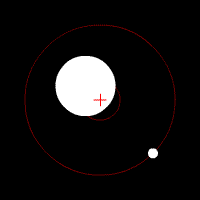
\includegraphics[width=0.4\textwidth]{radial-velocity/two-body-cm}
	\caption{Schematic of a star (upper-left) and planet (lower-right) orbiting a common center-of-mass.}\label{rv:fig:two-body-cm}
\end{figure}

Consider the picture in Figure~\ref{rv:fig:two-body-cm} and define $M_\textrm{p} = 0.5 M_\textrm{J}$ as the mass of the planet (the smaller object),  $M_\textrm{S} = 1.0 M_\textrm{Sun}$ as the mass of the star (the larger object), and $d = 0.0527\:$AU be the separation between the two. Assume the system is in a circular orbit.

\begin{steps}
	\item How far is the Center of Mass from the center of the star (in AU)?
	
	\item What is the star’s orbital radius (in AU)?
\end{steps}

Since the star is moving around the Center of Mass, it has a non-zero velocity. Let the orbital period of the system be $T = 4.23\:$days.

\begin{steps}
	\item What is the orbital velocity of the host star?
	
	\item Sketch the figure, then on that sketch, draw arrows showing the velocity at different parts of the orbit. What happens to the direction of the star’s velocity as the planet traces out its orbit?
\end{steps}

Astronomers can use spectroscopic techniques for measuring the velocity of stars along the line of sight between the earth and the star. In the illustration in Figure~\ref{rv:fig:two-body-cm}, suppose the earth is to the right of the system so that we are observing the system edge on from the right side of the page. \textbf{Draw a graph} similar to Figure~\ref{rv:fig:graph} and then draw on it the ``line of sight'' velocity for the star as a function of time (hint: it will be a trigonometric function).

\begin{figure}
	\centering
	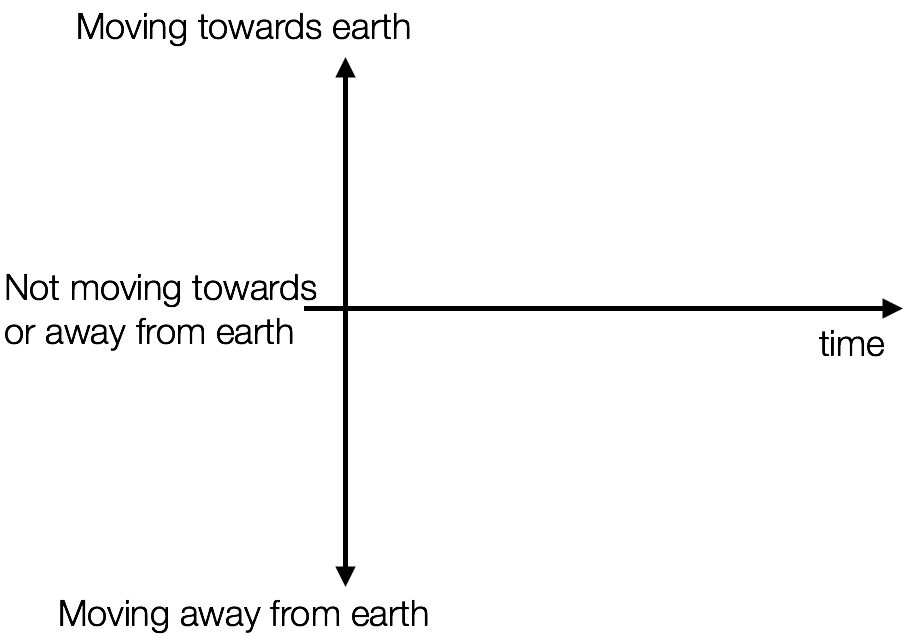
\includegraphics[width=0.6\textwidth]{radial-velocity/radial-graph}
	\caption{Graph to draw for radial velocity estimation.}\label{rv:fig:graph}
\end{figure}

\begin{steps}
	\item How are the period and amplitude related to the orbital period and the star’s velocity?
\end{steps}

Consider a similar system only with a planet that is twice the mass ($M_\textrm{p} = M_\textrm{J}, M_\textrm{S} = M_\textrm{Sun}$, $d = 0.0527\:$AU, and $T = 4.23\:$days).

\begin{steps}
	\item What is the system's host star orbital radius (in AU) and orbital velocity (in m/s)?
	
	\item How do these compare with the values for the previous system with a less massive planet?
\end{steps}

\textbf{Sketch the line of sight velocity} for this more massive system on the same plot that you already drew.

\begin{steps}
	\item How does the line of sight velocity depend on the planet’s mass?
\end{steps}

Open the link for the radial velocity simulator (\url{http://astro.unl.edu/naap/esp/animations/radialVelocitySimulator.html}). Under ``Visualization Controls'' click ``show multiple views.'' Under ``Planet Properties'' set the eccentricity to zero. Under ``Animation Controls,'' press ``Start Animation'' to set things in motion. Vary the mass of the planet, the mass of the star and the semimajor axis and note how the radial velocity graph changes. Vary the other parameters (eccentricity, longitude, inclination) and see how the radial velocity changes. \textbf{Include your findings in your report.}

\section{Radial velocity of 51 Peg}

Table~\ref{rv:tab:51peg} lists actual line of sight velocities for 51 Peg measured by Marcy \& Buttler in 1995 at the Lick Observatory in California.

\begin{table}
	\centering
	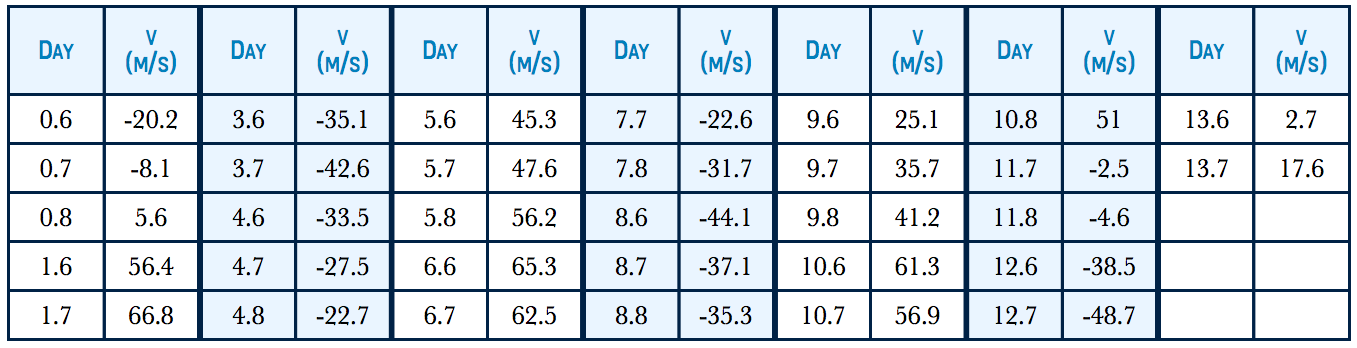
\includegraphics[width=\textwidth]{radial-velocity/51-peg-velocities}
	\caption{Line-of-sight velocities for 51 Pegasi measured over time.}\label{rv:tab:51peg}
\end{table}

Use the free software SciDAVis to plot this data. You can download and install it on your computer, or you can use the lab computers, which have it installed already.

Then, fit an equation to the data. To do so in SciDAVis, first save the project, so you won't accidentally lose your work. Then, select Analysis $\blacktriangleright$ Fit Wizard... from the drop-down menu. Type your desired equation into the large box. You can use any of the functions you can find in the lists at the top of the window and combine them how you would like. For fit parameters, use the letters a, b, c, and so on. For each fit parameter you use, include it in the list of parameters. For example, if you think the data are best represented by a tangent function, you could put ``\texttt{b*tan(c*x+d)}'' in the box. Then click the ``Fit $>>$'' button, then the ``Fit'' button to fit the data with this equation. This finds the parameters for the equation that make it best fit the data. Experiment to find an equation that seems to fit well.

You can retrieve the fit parameters and their uncertainties from the Results Log on the main window. \textbf{Include the graph, the fit parameters, and their uncertainties in your report.}

\begin{steps}
	\item From your fit to the data, what is the orbital period (days) and host star orbital velocity (m/s)?
	
	\item What is the orbital radius (in AU) for the host star?
\end{steps}

Kepler's third law relates the orbital period to the system's semimajor axis. In the case where the planet’s mass is much smaller than the star’s mass, Kepler's third law is
\begin{equation}
 P^2=\frac{4 \pi^2}{GM} a^3 \,,
\end{equation}
where $P$ is the orbital period, $G$ is Newton's constant, $M$ is the mass of the star, and $a$ is the semimajor axis. The mass of 51Peg is $1.0 M_\textrm{Sun}$.

\begin{steps}
	\item According to your fitted orbital period and Kepler's third law, what is the system's semimajor axis?
\end{steps}

The host star orbital radius and the semimajor axis are related by the Center of Mass.

\begin{steps}
	\item Using the system's semimajor axis, the mass of 51Peg, and the host star’s orbital period, determine the planet’s mass (in units of $M_\textrm{J}$).
\end{steps}

\section{Radial velocities for other systems}

Go to the webpage for SystemicLive (\url{http://www.stefanom.org/systemic-live/}). Note that while the graphics within the tutorial are currently not visible on the website, the data visualization and analysis software are still functional). Click ``Open Systemic'' to start the program. Then on that first page, scroll down to ``Tutorials and Resources'' and click on the link ``51 Pegged: Rediscovering the first exoplanet with Systemic Live'' and follow that tutorial. You will use the Systemic software to analyze radial velocity data for 51Peg.

Note that one key analysis tool you will use in the remainder of the lab is the power spectrum of the radial velocity data. We know that we can create any periodic function from the sum of sinusoids of different frequencies and phases. The power spectrum tells us which frequencies dominate that decomposition. Therefore, peaks in the power spectrum correspond to periodicities in the data, and hence point to possible planetary periods in the radial velocity measurements.

\begin{steps}
	\item How do the mass and separation results from Systemic compare with your earlier 51Peg numbers? Print out a plot of the ``Phased Radial Velocity'' and write on it the Period and Mass for the system.
	
	\item Use Systemic to determine orbit parameters for the following systems: 47Uma, 70Vir. Print out plots for your ``Phased Radial Velocity'' for each system. Write on your plots the Period and Mass for each system orbit.
	
	\item Use Systemic to analyze the data for system: upsand. Hint, there are multiple planets for this system. How many planets do you find? What are their masses and orbital periods?
	
\end{steps}

\section{Reflection}

Do some research on the history and background of the systems you analyzed (51Peg, 47Uma, 70Vir, and upsand). Write a one paragraph summary of this lab and discuss the following:

\begin{steps}
	\item What was the historical context and significance of these measurements?
	
	\item How do they relate to what you did in this lab?
\end{steps}
\chapter{Detecting exoplanets with the transit method}

\section{Part 1}

See other handout on Canvas for Part 1.

\section{Part 2}

Throughout the upcoming week, you will use    one    of    the    MicroObservatory    telescopes,    built    and    maintained    by    the    Harvard‐Smithsonian    Center    for    Astrophysics    and    located    at    the    Whipple    Observatory    in    Amado,    Arizona    to    take    a    series    of    images    of    a    ``target''    star in order to calculate a light curve for that star, which could be used to learn about the planet(s) orbiting them.    These    images    will    form    the    basis    of    your    subsequent    investigation in the Image Lab on the LSE website.

During this class, you will determine which stars you are imaging and decide among your group who will schedule the observations. After you do this, you will use the LSE website to analyze an example image, so you can analyze your own images later at home for the report.

The report will be due two weeks from today's lab, rather than one week, to account for the extra work at home.

\subsection{Scheduling observations}

Throughout the upcoming week, you will use    one    of    the    MicroObservatory    telescopes,    built    and    maintained    by    the    Harvard‐Smithsonian    Center    for    Astrophysics    and    located    at    the    Whipple    Observatory    in    Amado,    Arizona    to    take    a    series    of    images    of    a    ``target''    star.    These    images    will    form    the    basis    of    your    subsequent    investigation in the Image Lab on the LSE website.

Log on to LSE using the credentials emailed to you and click “Go to the
Lab.”

Click on the “Telescope” tab and go through the sections on the right
side of the page to learn about the remote observatory we are using and
how to schedule observations.
%\textit{Note: you can only schedule observations
%for the current night and the schedule times are Chicago time.}

Next, look at the transit calendar file posted on the canvas course
website, “2019\_April\_May\_transit\_calendar.pdf,” which lists observable
transits by the remote observatory each night. Note, times are for
Tucson, AZ, not Chicago. Work out with your TA and rest of the section a
plan for observing a few transits over the course of the week. Each
transit will require observing for $\sim 1$ hour before and $\sim 1$ hour after the
transit for a total observation time of 4--5 hours. This corresponds to 80--
100 exposures. One possible arrangement would be to have smaller
groups responsible for scheduling different segments of the total
observation, e.g.: group 1 can schedule observing for the 1st hour, group
2 would schedule the second hour, etc\dots{} Make plans for observing a
number of systems throughout the week. If possible, conduct multiple
observations of the same system. \textit{Note: you can only schedule
observations for the current night, so you will need to login and
schedule your observations on the appropriate day of the week.}

Once your observations have been completed, you can analyze them on
your own, but in lab we will practice this analysis with example data.

Click on the “Image Lab” and go through the 9 page tutorial. Practice
your analysis on the “Demo\_Images” for TRES-3. Make sure you subtract
and appropriate Dark Image (note that the image filenames include the
date and time of the exposure).

Once it’s been taken, analyze the data from your scheduled
observations. Be sure to press the “Calculate \& Record” button to save
your results.

Combine your data with the rest of the sections (you might have to re-
do the previous week’s activities) by looking at the “class graph.” \textbf{Save this light curve and turn it in with your write up.}

\section{Report checklist and grading}

Each item below is worth 10 points, and there is an additional 10 points for attendance and participation.

\begin{itemize}
	\item Data table from Part 1.
	
	\item Plots of your light curves for Planet 1, Planet 2, and all of the planets you observed with LSE. 
	
	\item Discuss how different features of the light curve connected to physical
	properties of the orbital system.
	
	\item What is your interpretation of the
	temperatures for the simulated planets (Planet 1 \& 2)?
	
	\item List which scheduled observations your group performed. Were you able to see a light curve from your scheduled observations? Why or why not?
\end{itemize}
\chapter{Using Kepler’s Laws to find the density of Jupiter}

%todo include caution about rotation of image compared to website
%todo give the density of water, to aid analysis of planet as rocky or gaseous

\section{Introduction}

So far, you have been using several techniques to learn about the properties of planets orbiting other stars based one what we can observe from Earth, including using orbital properties to discover the mass of planets. The same physical laws can be used to study planets and their moons.

To study the composition of a planet, it is useful to know its density --- then one can learn more about whether it is rocky or gaseous. In this lab, you will use Kepler's Laws to find the density of Jupiter, given orbital properties of its moons. In this case, we can use actual images of the these using Stone Edge Observatory, a remotely operated telescope in California.

Under nominal circumstances, we would have you schedule the observations yourself, so you could analyze the data that you, yourself, took. However, the observatory is not operating well enough right now to let that happen. Fortunately, we have archival images that were taken in 2017 by this observatory that you can analyze.

\section{Team roles}

\begin{steps}
	\item \textbf{Decide on roles} for each group member.
\end{steps}

The available roles are:
\begin{itemize}
	\item Facilitator: ensures time and group focus are efficiently used
	\item Scribe: ensures work is recorded
	\item Technician: oversees apparatus assembly, usage
	\item Skeptic: ensures group is questioning itself
\end{itemize}

These roles can rotate each lab, and you will report at the end of the lab report on how it went for each role. Some members will be holding more than one role. For example, you could have the skeptic double with another role. Consider taking on a role you are less comfortable with, to gain experience and more comfort in that role.

Additionally, if you are finding the lab roles more restrictive than helpful, you can decide to co-hold some or all roles, or think of them more like functions that every team needs to carry out, and then reflecting on how the team executed each function.

\section{Add members to Canvas lab report assignment group}

\begin{steps}
	\item On Canvas, navigate to the People section, then to the ``Lab 4 Groups'' tab. Find a group that is not yet used, and have each person in your group add themselves to that same lab group.
\end{steps}

This enables group grading of your lab report. Only one person will submit the group report, and all members of the group will receive the grade and have access to view the graded assignment.

\section{Using Kepler's laws}

Keplers third law relates the orbital period to the systems semi-major axis. In the case where the planets mass is much smaller than the stars mass, Kepler's third law is:
\begin{equation}
P^2 = \frac{4\pi^2}{G M}a^3 \,,
\end{equation}
where $P$ is the orbital period, $G$ is Newton's constant ($6.674 \times 10^{-11}\:\textrm{N}\:\textrm{m}^2/\textrm{kg}^2$), $M$ is the mass of Jupiter, and $a$ is the semi-major axis.

We can rewrite the third law as:

\begin{equation}
\frac{a^3}{P^2} = \frac{G}{4\pi^2}\left(\frac{4}{3}\pi R^3\rho \right) = \rho\frac{G R^3}{3\pi}
\end{equation}

where $R$ is the radius of Jupiter and $\rho$ (the Greek letter pronounced ``row'') is the density of Jupiter. Solving for $\rho$ gives:

\begin{equation}\label{jd:eqn:kepden}
\rho = \left(\frac{a}{R}\right)^3\frac{3\pi}{G P^2}
\end{equation}

The goal for this lab is to use our data to determine the ratio $(a/R)$ for each moon. We can then combine that with the moons period to estimate the density of Jupiter.

To determine the semi-major axis, $a$, for a moon's orbit, we can assume that the orbit is actually a circular orbit, and we know that we are viewing the orbits edge-on. So what we are seeing is a projection of a circular motion onto one dimension, which results in a sinusoidal motion, with the amplitude of that motion being the radius of the orbit (and thus the semi-major axis). So here we will analyze images taken at different times, plot the angular position of the moon over time, fit those data points to a sine (or, equivalently, a cosine) function, and the amplitude will be the semi-major axis, $a$.

\section{The set of observations}

The images can be found on Canvas, in the Files section, in the compressed file ``jupiter\_data.zip''.

Observations were taken on four separate dates between April 14 and 23, 2017, as stated in the names of the files. Images were taken in each of the \textit{g}, \textit{r}, \textit{i}, and \textit{clear} bands. These refer approximately to the color filters used in each case: green, red, infrared, and  clear (no filter). See Figure~\ref{jd:fig:filters} for the frequency response of such a filter set. All images were taken with a $0.05\:$second exposure time.

\begin{figure}
	\centering
	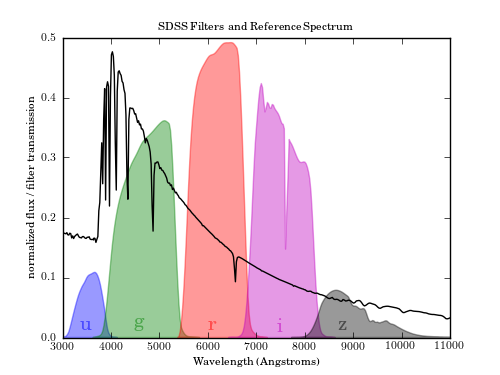
\includegraphics[width=0.8\textwidth]{jupiter-density/fig_sdss_filters_1}
	\caption{Typical transmission rates of various filters used in astronomy. This is from the Sloan Digital Sky Survey.}\label{jd:fig:filters}
\end{figure}

%\section{Make color images}
%
%All CCDs which are used in astronomical images are monochrome --- they do not have different pixels for different wavelengths of light, which allows them to achieve higher resolution. To create a color image, we must combine the images taken with different color filters and add color ourselves.
%
%One can easily make RGB images in DS9 by selecting \textit{Frame} $>$ \textit{New Frame RGB}, which allows one to upload different .fits files for each color with \textit{File} $>$ \textit{Open} depending on the color selected in the pop-up window. You can then scale each image as needed to make 3-color images. \textbf{Make an RGB image for Jupiter.}
%
\section{Analysis}

You will use the \textit{clear} images to measure the position of the moons relative to Jupiter and
\textit{gri} images to measure the radius of Jupiter. Since we will be using the ratio of moon position to Jupiter radius, we can use whatever units are convenient to measure the distance, as long as we are consistent, as the unit divides by itself in the calculation.

\begin{steps}
	
	\item Download and install DS9 from \url{http://ds9.si.edu/site/Download.html}. SAOImage DS9, or DS9 for short, is an image viewer, analyzer, and processor written and used by astronomers for working with astronomical images.
	
	If you click the link to download, it might say "redirecting" while never actually redirecting. In this case, copy the link into the address bar directly.
	\begin{framed}	
		\textbf{For MacOS}, unless you know otherwise, choose from the top set of choices (to the right of
		the blue apple logo). To find your version, from the Apple menu in the corner of the screen,
		choose “About This Mac”.
		
		If it displays a warning and prevents you from installed from an unidentified developer, follow the instructions at the following link to create an exception:
		
		\url{https://support.apple.com/guide/mac-help/open-a-mac-app-from-an-unidentified-developer-mh40616/mac}
	\end{framed}

	\item Open the Google Sheet found here: \url{https://docs.google.com/spreadsheets/d/1y1vfi3l1KzGoE0cOctwA0Z5s7ioptaRFpSLItBoRv2c/edit?usp=sharing}
	
	\item Make a copy of this sheet for your group to use. Explore the parts of the sheet. Notice the model equation and fit parameters at the top. Notice the data columns, including the time, distance from the center of Jupiter \texttt{x}, and the radius of Jupiter \texttt{R\_Jupiter}. There is also a plot of the measured and model $x/R$. There is a different sheet for each moon you are observing. Notice the different tabs at the bottom of the window for each of the four moons.
	
	\item Download the Jupiter data zip file from Canvas and extract it to a folder on your computer.
	
	\item Start DS9 and open the file from the earliest timestamp, with the clear filter.
	
	\item \textbf{Record the time} the image was taken by going to the \textit{File} menu and then \textit{Display Fits Header}. Towards the bottom of the header will be listed the \textit{DATE-OBS} which will be in the UTC timezone.
	
	\item Convert the time given to decimal time in days after 2017-04-14T00:00:00. It may help to use the converter below the plot in the spreadsheet.
\end{steps}

In the data table, there is an entry for each tenth of a day, so that the model $x/R$ can be computed and plotted.

\begin{steps}
	\item To include your measurement, insert a new row for the image's timestamp by right-clicking the row number of the time just before the image's timestamp and selecting ``Insert 1 below''.
	
	\item Enter your image's decimal time in the time column.

	\item Identify the moons in your image by doing the following:
	\begin{enumerate}
		\item Adjust the contrast and zoom in your image until you can clearly see Jupiter and four moons. To get a better view, select ``Scale $>>$ Log'' from the drop-down menus, and also right-click-drag up, down, left, and right anywhere on the image to adjust the contrast dynamically.
		
		\item In another browser tab, open \url{http://www.shallowsky.com/jupiter/}, enter the observation time, and press the circular arrow ``refresh'' symbol. It automatically adjusts for your local timezone (in Chicago it adds ``-5'' to the end of the timestamp.), so to unadjust back to UTC, do that arithmetic operation to the entered time. In the case of Chicago and ``-5'', subtract 5 hours from the entered time.
		
		\item Ensure the images match and correct the time if necessary. If the image seems flipped or rotated, select a different orientation from the drop-down.
	\end{enumerate}
	
	\item \textbf{Use} DS9 to measure the distance from the center of Jupiter to each moon using the Ruler function described in the following paragraph. Keep track of whether the moon is on the East or West side of Jupiter by making all locations on the left side positive and locations on the right side negative. \textbf{Record your value} in the data table for each moon.
\end{steps}

You can use the DS9 \textit{Ruler} function to measure the distance (in pixels) between two points in the image. To use the \textit{Ruler}, first go to the Region menu from the toolbar at the top. Select the \textit{Shape} sub-menu and click \textit{Ruler}. Then, click the \textit{Edit} menu button and select \textit{Region}. You can then use the mouse to draw a line between two points and DS9 will calculate the distance for you. If you have trouble using the \textit{Ruler} feature, you can also read off the $(x,y)$ coordinates for each point and calculate the distance yourself using Pythagorean's theorem.

\begin{steps}
	\item Repeat the above analysis for each of the four timestamps.
\end{steps}

The apparent radius of Jupiter can be different for each image, since the apparent brightness can change depending on local weather conditions. So if available, you will measure its radius for each timestamp.

\begin{steps} 
	\item For each timestamp, if its available, load the image taken with the ``i'' filter, listed in the filename, and measure Jupiter's radius, recording it in the table. If there is no such image, take an average of the other image's measured radii.
\end{steps}

You should now have 4 distances for each of the four moons recorded in their respective data tables. Now you will plot them and fit the sine functions, to find the semi-major axis of each one.

\section{Plotting and fitting}

\begin{steps}
	\item For each row of measured data, enter the formula for the ``$x/R$ measured'' row. In Google Sheets, the procedure is as follows:
	\begin{enumerate}
		\item Select the cell in which you want to enter the formula (to the right of your measured \texttt{R\_Jupiter}.)
		
		\item Enter ``\texttt{=}'', click the cell that contains your measured $x$ to insert that cell's identifier, enter ``/'', click the cell that contains your measured $R_J$, and press enter. Ensure that it divided the correct values.
	\end{enumerate}

	\item In the next column, marked ``x/R model'', you need to continue the formula from the row above, in order to computer the model x/R for that timestamp. To do this, click on the cell in the row above, then click and drag the box on the lower right of the cell's border down by one cell.
	
	\item Do the same for the \texttt{diff\^{}2} column.
\end{steps}

Now you should have all four data points displaying on the plot, for each moon, and you are ready to fit the sine curve for each moon, so you can find the ratio semi-major axis divided by Jupiter radius, $a/R$, as needed for applying Kepler's third law as in Equation\ \ref{jd:eqn:kepden}.

\begin{steps}
	\item For each moon, enter the period of its orbit (from Table\ \ref{jd:tab:periods}) in the fit parameter for period, \texttt{B}.
	
	\item For each moon, adjust the other fit parameters, amplitude and time offset, to visually match the measured points, and then fine-adjust to minimize the rms deviation.
\end{steps}

\begin{table}
	\centering
	\begin{tabular}{ l c r }
		\hline
		Moon & Period (days) & $\rho_\textrm{Jupiter}$ $(\textrm{kg/m}^3)$\\
		\hline
		Ganymede & 7.1546 & \\
		Io & 1.7691 & \\
		Europa & 3.5512 & \\
		Calisto & 16.689 & \\
		\hline  
	\end{tabular}
	\caption{Four moons of Jupiter and their periods.}\label{jd:tab:periods}
\end{table}

The amplitude from your fit corresponds to the ratio, $(a/R)$ which we will use in Kepler’s Third law.

\begin{steps}
	\item For each moon, use the amplitude of the curve together with Kepler's Third law
	to estimate the density of Jupiter. Make sure you use the right units for your values. \textit{Hint:
	look at the units for the Gravitational constant. What units do you need for the moons
	orbital period?}

	\item\label{jd:step:density} Take the average of the densities, and use the standard deviation of them for the uncertainty. Report this value, with uncertainty, in your report.
	
	\item Compare your result to a value of the density you find online, using the uncertainties and the procedure in Appendix~\ref{unc:sec:comparing}. How close are they? What are possible sources of uncertainty of your measurement?
	
	\item\label{jd:step:composition} Rocky planets in our solar system have densities ranging from 3000--5000$\:$kg/m$^3$, and water has a density of 1000$\:$kg/m$^3$ (atmospheric air at sea level on Earth has a density of about 1$\:$kg/m$^3$). Given these ranges and your result, would you conclude that Jupiter is rocky or gaseous, and why?
\end{steps}

\section{Report checklist and grading}

Each item below is worth 10 points, and there is an additional 10 points for attendance and participation.

\begin{enumerate}
	\item Data table including times and positions for each moon, as well as the radius of Jupiter.
	
	\item Graphs of position ($x/R$) vs. time for each moon, with the fitted curve plotted as well.
	
	\item Answers or evidence of completion for Steps~\ref{jd:step:density}--\ref{jd:step:composition}.
	
	\item A 100--200 word reflection on group dynamics and feedback on the lab manual. Address the following topics: who did what in the lab, how did you work together, what successes and challenges in group functioning did you have, and what would you keep and change about the lab write-up?
	
\end{enumerate}

\appendix

% This format is not a formal report, but simply answering questions, including figures, and demonstrating scientific abilities.
\chapter{Lab Report Format}\label{cha:lab-report-format}

%TODO Make firm page limit? 5 pages + figures and tables?

%In a general sense, the labs should demonstrate the rubric rows listed in the lab write-up and provide answers to every lab question asked.

\section{General}

\begin{itemize}
	\item The report should be typed for ease of reading. Text should be double-spaced, and the page margins (including headers and footers) should be approximately $2.5\:$cm, for ease of marking by the grader. Each page should be numbered.
	
	\item The first page should include the title of the lab; lab section day, time, and number; and the names of the members of your lab team.
	
%	\item If the rubric row refers to a particular part of your lab report, clearly label that part of the report with that rubric row. For example, you should label the section where you demonstrate uncertainty propagation with ``G2'' if that rubric row is being assessed in that lab.
\end{itemize}

\section{Organizing the report}

%If the lab is clearly framed as an observational, testing, or application experiment, you can follow the corresponding rubric for the elements to include in the report (see, respectively, Rubrics B, C, and D in Appendix~\ref{cha:rubrics}).

The report should follow the sequence of the report checklist. Answers to questions and inclusion of tables and figures should appear in the order they are referenced in the manual. In general, include the following:

	\begin{itemize}
%		\item Any procedure that you performed that is different from what is described in the lab manual.
		
%		\item Any data that you've collected: tables, figures, measured values, sketches. Whenever possible, include an estimate of the uncertainty of measured values.
		
		\item For any calculations that you perform using your data, and the final results of your calculation, you must show your work in order to demonstrate to the grader that you have actually done it. Even if you're just plugging numbers into an equation, you should write down the equation and all the values that go into it. This includes calculating uncertainty and propagation of uncertainty.
		
		\item If you are using software to perform a calculation, you should explicitly record what you've done. For example, ``Using Excel we fit a straight line to the velocity vs. time graph. The resulting equation is $v = (0.92\:\mathrm{m/s^2}) t + 0.2\:\mathrm{m/s}$.''
		
		\item Answers to any questions that appear in the lab handout. Each answer requires providing justification for your answer.
		
%		\item At the end of each experiment, you should discuss the findings and reflect deeply on the quality and importance of the findings%
		% (Rubric Row F2)
%		. This can be both in the frame of a scientist conducting the experiment (``What did the experiment tell us about the world?'') and in the frame of a student (``What skills or mindsets did I learn?'').
	\end{itemize}

\section{Graphs, Tables, and Figures}

Any graph, table, or figure (a figure is any graphic, for example a sketch) should include a caption describing what it is about and what features are important, or any helpful orientation to it. The reader should be able to understand the basics of what a graph, table, or figure is saying and why it is important without referring to the text. For more examples, see any such element in this lab manual.

Each of these elements has some particular conventions.

\subsection{Tables}

A table is a way to represent tabular data in a quantitative, precise form. Each column in the table should have a heading that describes the quantity name and the unit abbreviation in parentheses. For example, if you are reporting distance in parsecs, then the column heading should be something like ``distance (pc)''. This way, when reporting the distance itself in the column, you do not need to list the unit with every number.

\subsection{Graphs}

A graph is a visual way of representing data. It is helpful for communicating a visual summary of the data and any patterns that are found.

The following are necessary elements of a graph of two-dimensional data (for example, distance vs. time, or current vs. voltage) presented in a scatter plot.

\begin{itemize}
	\item \textbf{Proper axes.} The conventional way of reading a graph is to see how the variable on the vertical axis changes when the variable on the horizontal axis changes. If there are independent and dependent variables, then the independent variable should be along the horizontal axis.
	
	\item \textbf{Axis labels.} The axes should each be labeled with the quantity name and the unit abbreviation in parentheses. For example, if you are plotting distance in parsecs, then the axis label should be something like ``distance (pc)''.
	
	\item \textbf{Uncertainty bars.} If any quantities have an uncertainty, then these should be represented with so-called ``error bars'', along both axes if present. If the uncertainties are smaller than the symbol used for the data points, then this should be explained in the caption.

\end{itemize}

\chapter{Analysis of Uncertainty}

A physical quantity consists of a value, unit, and uncertainty.
For example, ``$5 \pm 1\,$m'' means that the writer believes the true value of the quantity to most likely lie within 4 and 6 meters\footnote{The phrase ``most likely'' can mean different things depending on who is writing.
	If a physicist gives the value and does not given a further explanation, we can assume that they mean that the measurements are randomly distributed according to a normal distribution around the value given, with a standard deviation of the uncertainty given.
	So if one were to make the same measurement again, the author believes it has a 68\% chance of falling within the range given.
	Disciplines other than physics may intend the uncertainty to be 2 standard deviations.}.
Without knowing the uncertainty of a value, the quantity is next to useless.
For example, in our daily lives, we use an implied uncertainty.
If I say that we should meet at around 5:00 pm, and I arrive at 5:05 pm, you will probably consider that within the range that you would expect.
Perhaps your implied uncertainty is plus or minus 15 minutes.
On the other hand, if I said that we would meet at 5:07 pm, then if I arrive at 5:10 pm, you might be confused, since the implied uncertainty of that time value is more like 1 minute.

Scientists use the mathematics of probability and statistics, along with some intuition, to be precise and clear when talking about uncertainty, and it is vital to understand and report the uncertainty of quantitative results that we present.

\section{Types of measurement uncertainty}

For simplicity, we limit ourselves to the consideration of two types of uncertainty in this lab course, instrumental and random uncertainty.

\subsection{Instrumental uncertainties}

Every measuring instrument has an inherent uncertainty that is determined by the precision	
  of the instrument.
Usually this value is taken as a half of the smallest increment of the instrument's scale. For example, $0.5\:$mm is the precision of a standard metric ruler; $0.5\:$s is the precision of a watch, etc. For electronic digital displays, the equipment's manual often gives the instrument's resolution, which may be larger than that given by the rule above.

Instrumental uncertainties are the easiest ones to estimate, but they are not the only source of the uncertainty in your measured value.
You must be a skillful experimentalist to get rid of all other sources of uncertainty so that all that is left is instrumental uncertainty.

\subsection{Random uncertainties}

Very often when you measure the same physical quantity multiple times, you can get different results each time you measure it.
That happens because different uncontrollable factors affect your results randomly.
This type of uncertainty, random uncertainty, can be estimated only by repeating the same measurement several times.
For example if you measure the distance from a cannon to the place where the fired cannonball hits the ground, you could get different distances every time you repeat the same experiment.	
  
For example, say you took three measurements and obtained 55.7, 49.0, 52.5, 42.4, and 60.2 meters. We can quantify the variation in these measurements by finding their standard deviation using a calculator, spreadsheet, or the formula (assuming the data distributed according to a normal distribution)
\begin{equation}
 \sigma = \sqrt{\sum_{i=1}^{N} \frac{(x_i-\bar{x})^2}{N-1}} \, ,
\end{equation}
where $\{x_1, x_2, \dots, x_N\}$ are the measured values, $\bar{x}$ is the mean of those values, and $N$ is the number of measurements.
For our example, the resulting standard deviation is 6.8 meters. Generally we are interested not in the variation of the measurements themselves, but how uncertain we are of the average of the measurements. The uncertainty of this mean value is given, for a normal distribution, by the so-called ``standard deviation of the mean'', which can be found by dividing the standard deviation by the square root of the number of measurements,
\begin{equation}
\sigma_\textrm{mean} = \frac{\sigma}{\sqrt{N}} \, .
\end{equation}
So, in this example, the uncertainty of the mean is 3.0 meters. We can thus report the length as $52 \pm 3\:$m.

Note that if we take more measurements, the standard deviation of those measurements will not generally change, since the variability of our measurements shouldn't change over time. However, the standard deviation of the mean, and thus the uncertainty, will decrease.

\section{Propagation of uncertainty}

When we use an uncertain quantity in a calculation, the result is also uncertain. To determine by how much, we give some simple rules for basic calculations, and then a more general rule for use with any calculation which requires knowledge of calculus. Note that these rules are strictly valid only for values that are normally distributed, though for the purpose of this course, we will use these formulas regardless of the underlying distributions, unless otherwise stated, for simplicity.

If the measurements are completely independent of each other, then for quantities $a \pm \delta a$ and $b \pm \delta b$, we can use the following formulas:
\begin{equation}\label{unc:add}
\textrm{For } c = a + b \textrm{ (or for subtraction), } \delta c = \sqrt{(\delta a)^2 + (\delta b)^2}
\end{equation}

\begin{equation}\label{unc:mult}
\textrm{For } c = ab \textrm{ (or for division), } \frac{\delta c}{c} = \sqrt{\left(\frac{\delta a}{a}\right)^2 + \left(\frac{\delta b}{b}\right)^2}
\end{equation}

\begin{equation}\label{unc:exp}
\textrm{For } c = a^n,\, \frac{\delta c}{c} = n \frac{\delta a}{a}
\end{equation}

If you are familiar with calculus, you may want to use this general formula for the uncertainty $\delta f$ of a function $f$ of $N$ independent values $x_i$, each with uncertainty $\delta x_i$:
\begin{equation}\label{unc:general}
\delta f = \sqrt{ \sum_{i=1}^{N} \left(\frac{\partial f}{\partial x_i} \delta x_i\right)^2 } \, .
\end{equation}
Notice that Eqs.\ \ref{unc:add} through \ref{unc:exp} can be derived from Eq.\ \ref{unc:general} for those specific cases.

\subsubsection{What if there is no reported uncertainty?}

Sometimes you'll be calculating with numbers that have no uncertainty given.
In some cases, the number is exact.
For example, the circumference $C$ of a circle is given by $C = 2 \pi r$. Here, the coefficient, $2\pi$, is an exact quantity and you can treat its uncertainty as zero.
If you find a value that you think is uncertain, but the uncertainty is not given, a good rule of thumb is to assume that the uncertainty is half the right-most significant digit.
So if you are given a measured length of $1400\:$m, then you might assume that the uncertainty is $50\:$m.
This is an assumption, however, and should be described as such in your lab report.
For more examples, see Table~\ref{unc:tab:implied}.

\begin{table}
	\begin{center}
		\begin{tabular}{cc}
			\textbf{Expression} & \textbf{Implied uncertainty} \\
			12 & 0.5 \\
			12.0 & 0.05 \\
			120 & 5 \\
			120. & 0.5
		\end{tabular}
		\caption{Expression of numbers and their implied uncertainty.}\label{unc:tab:implied}
	\end{center}
\end{table}

\subsubsection{How many digits to report?}

After even a single calculation, a calculator will often give ten or more digits in an answer.
For example, if I travel $11.3 \pm 0.1\:$km in $350 \pm 10\:$s, then my average speed will be the distance divided by the duration. Entering this into my calculator, I get the resulting value ``\texttt{0.0322857142857143}''.
Perhaps it is obvious that my distance and duration measurements were not precise enough for all of those digits to be useful information.
We can use the propagated uncertainty to decide how many decimals to include.
Using the formulas above, I find that the uncertainty in the speed is given by my calculator as ``\texttt{9.65683578099600e-04}'', where the `\texttt{e}' stands for ``times ten to the''.
I definitely do not know my uncertainty to 14 decimal places.
For reporting uncertainties, it general suffices to use just the 1 or 2 left-most significant digits, unless you have a more sophisticated method of quantifying your uncertainties.
So here, I would round this to 1 significant digit, resulting in an uncertainty of $0.001\:$km/s.
Now I have a guide for how many digits to report in my value.
Any decimal places to the right of the one given in the uncertainty are distinctly unhelpful, so I report my average speed as ``$0.032 \pm 0.001\:$km/s''.
You may also see the equivalent, more succinct notation ``$0.032(1)\:$km/s''.

\section{Comparing two values}\label{unc:sec:comparing}

If we compare two quantities and want to find out how different they are from each other, we can use a measure we call a $t'$ value (pronounced ``tee prime''). This measure is not a standard statistical measure, but it is simple and its meaning is clear for us.

Operationally, for two quantities having the same unit, $a \pm \delta a$ and $b \pm \delta b$, the measure is defined as\footnote{Statistically, if $\delta a$ and $\delta b$ are uncorrelated, random uncertainties, then $t'$ represents how many standard deviations the difference $a - b$ is away from zero.}

\begin{equation}
%t' = \frac{\abs{a-b}}{\sqrt{(\delta a)^2 + (\delta b)^2}}
t' = \frac{\abs{a-b}}{\sqrt{(\delta a)^2 + (\delta b)^2}}
\end{equation}

If $t' \lesssim 1$, then the values are so close to each other that they are indistinguishable. It is either that they represent the same true value, or that the measurement should be improved to reduce the uncertainty.

If $1 \lesssim t' \lesssim 3$, then the result is inconclusive. One should improve the experiment to reduce the uncertainty.

If $t' \gtrsim 3$, then the true values are very probably different from each other.
%\begin{landscape}
\chapter{Rubrics}
	
	\freetabcaption{Rubric B: Ability to design and conduct an observational experiment \cite{etkina_scientific_2006}.}
	\begin{longtable}{>{\bfseries}p{0.02\textheight}|>{\bfseries\RaggedRight}p{0.25\textheight}|>{\RaggedRight}p{0.21\textheight}|>{\RaggedRight}p{0.21\textheight}|>{\RaggedRight}p{0.22\textheight}|>{\RaggedRight}p{0.22\textheight}}
		\toprule
		& Scientific Ability
		& Missing & Inadequate & Needs Improvement & Adequate \\ \midrule \endhead
		B1
		& Is able to identify the phenomenon to be investigated
		& No phenomenon is mentioned
		& The description of the phenomenon to be investigated is confusing, or it is not the phenomenon of interest.
		& \midsloppy The description of the phenomenon is vague or incomplete.
		& The phenomenon to be investigated is clearly stated. \\ \midrule
		B2
		& Is able to design a reliable experiment that investigates the phenomenon
		& The experiment does not investigate the phenomenon.
		& The experiment may not yield any interesting patterns.
		& Some important aspects of the phenomenon will not be observable.
		& The experiment might yield interesting patterns relevant to the investigation of the phenomenon. \\ \midrule
		B3
		& Is able to decide what physical quantities are to be measured and identify independent and dependent variables
		& The physical quantities are irrelevant.
		& Only some of physical quantities are relevant.
		& The physical quantities are relevant. However, independent and dependent variables are not identified.
		& The physical quantities are relevant and independent and dependent variables are identified. \\ \midrule
		B4
		& Is able to describe how to use available equipment to make measurements
		& At least one of the chosen measurements cannot be made with the available equipment.
		& All chosen measurements can be made, but no details are given about how it is done.
		& All chosen measurements can be made, but the details of how it is done are vague or incomplete.
		& All chosen measurements can be made and all details of how it is done are clearly provided. \\ \midrule
		B5
		& Is able to describe what is observed without trying to explain, both in words and by means of a picture of the experimental setup.
		& No description is mentioned.
		& A description is incomplete. No labeled sketch is present. Or, observations are adjusted to fit expectations.
		& A description is complete, but mixed up with explanations or pattern. Or the sketch is present but is difficult to understand.
		& Clearly describes what happens in the experiments both verbally and with a sketch. Provides other representations when necessary (tables and graphs). \\ \midrule
		B6
		& Is able to identify the shortcomings in an experiment and suggest improvements
		& No attempt is made to identify any shortcomings of the experiment.
		& The shortcomings are described vaguely and no suggestions for improvement are made.
		& Not all aspects of the design are considered in terms of shortcomings or improvements.
		& All major shortcomings of the experiment are identified and reasonable suggestions for improvement are made. \\ \midrule
		B7
		& Is able to identify a pattern in the data
		& No attempt is made to search for a pattern.
		& The pattern described is irrelevant or inconsistent with the data.
		& The pattern has minor errors or omissions. Terms like ``proportional'' used without clarity, e.g.\ is the proportionality linear, quadratic, etc.
		& The pattern represents the relevant trend in the data. When possible, the trend is described in words. \\ \midrule
		B8
		& Is able to represent a pattern mathematically (if applicable)
		& No attempt is made to represent a pattern mathematically.
		& The mathematical expression does not represent the trend.
		& No analysis of how well the expression agrees with the data is included, or some features of the pattern are missing.
		& The expression represents the trend completely and an analysis of how well it agrees with the data is included. \\ \midrule
		B9
		& Is able to devise an explanation for an observed pattern
		& No attempt is made to explain the observed pattern.
		& An explanation is vague, not testable, or contradicts the pattern.
		& An explanation contradicts previous knowledge or the reasoning is flawed.
		& A reasonable explanation is made. It is testable and it explains the observed pattern. \\
		\bottomrule
	\end{longtable}

	
%\end{table}

\end{landscape}

%\chapter{Manual: PASCO Cavendish Balance}\label{cha:pasco-cavendish}

On the following pages is the manual for the PASCO Cavendish Balance.

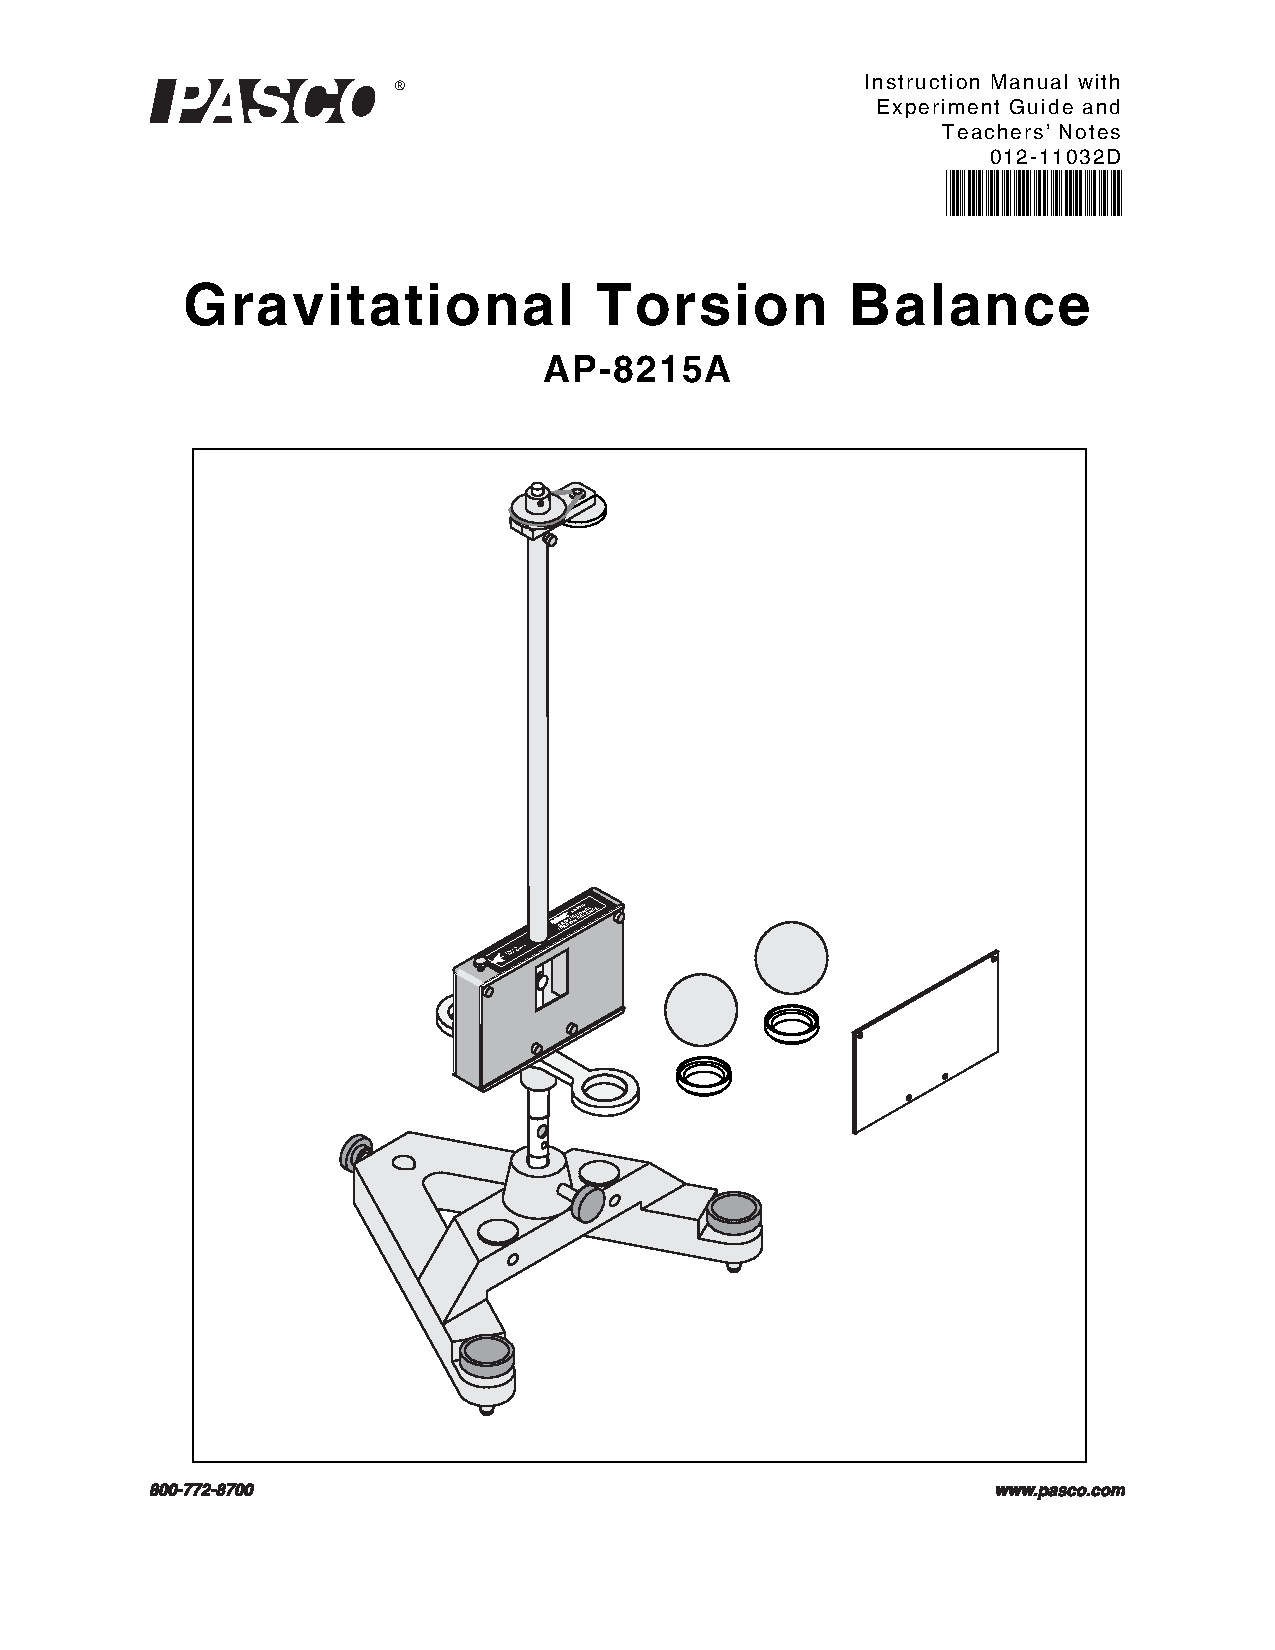
\includepdf[pages={1,3-8,16}]{pasco-cavendish/Gravitational-Torsion-Balance-Manual-AP-8215A.pdf}

% \bibliography{references,MyLibrary}
% \bibliographystyle{plain}
\printbibliography

\end{document}
